\chapter{Problem Statement and Proposed Solution}

\pagebreak

\section{Problem Statement}

Narrative therapy is embracing into the second decade on the arena of psychotherapy. Yet, how can these therapeutic qualities best be inferred? How persuasive are the arguments relating to its effectiveness? What type of work is presides over with patients that portray that such practices are indeed beneficial to people? And lastly, how solid is the narrative-inspired research(often called co-research) that forge the use of externalizing practices? A distinctive quality of the therapeutic stance, if narrative therapy lies in the manner in which it pledges from the postmodern philosophical tradition. Similarly, narrative-based research pop up to be unique from other genre of research in mental health professions.

Conventional forms of research generally search for empirical conclusions (as with quantitative designs) and consistently rely on the researcher’s expert role to collect, codify, and interpret data (as is the case with many forms of qualitative methodology). Narrative-inspired research, conversely, limelight’s on the subjective nature of experience and inquire to de-emphasize the therapist’s role as an expert.

The relevant elements necessary for a basic psychotherapy reading, is:
\begin{itemize}
    \item What the main problem is (for example depression or anxiety).
    \item What triggers it (what makes the patient feel that way on a day to day basis).
    \item Examples of patient's symptoms, changes in patients behaviours and thinking.
    \item What consequence the problem has on patient's life.
\end{itemize}

An example with all the relevant elements needed, is:
``My main problem is feeling depressed most of the day every day. I feel tired, my Appetite is affected and I struggle to concentrate. I have stopped seeing friends, goingto work or doing things around the home and I am spending more time in bed. I have thoughts that I am letting my family down and that I can't be bothered. As a Consequence, I am isolated and being off sick means I have used up most of my savings and money is tight''.

\section{Existing State of the Art}

\begin{figure}[H]
    \centering
    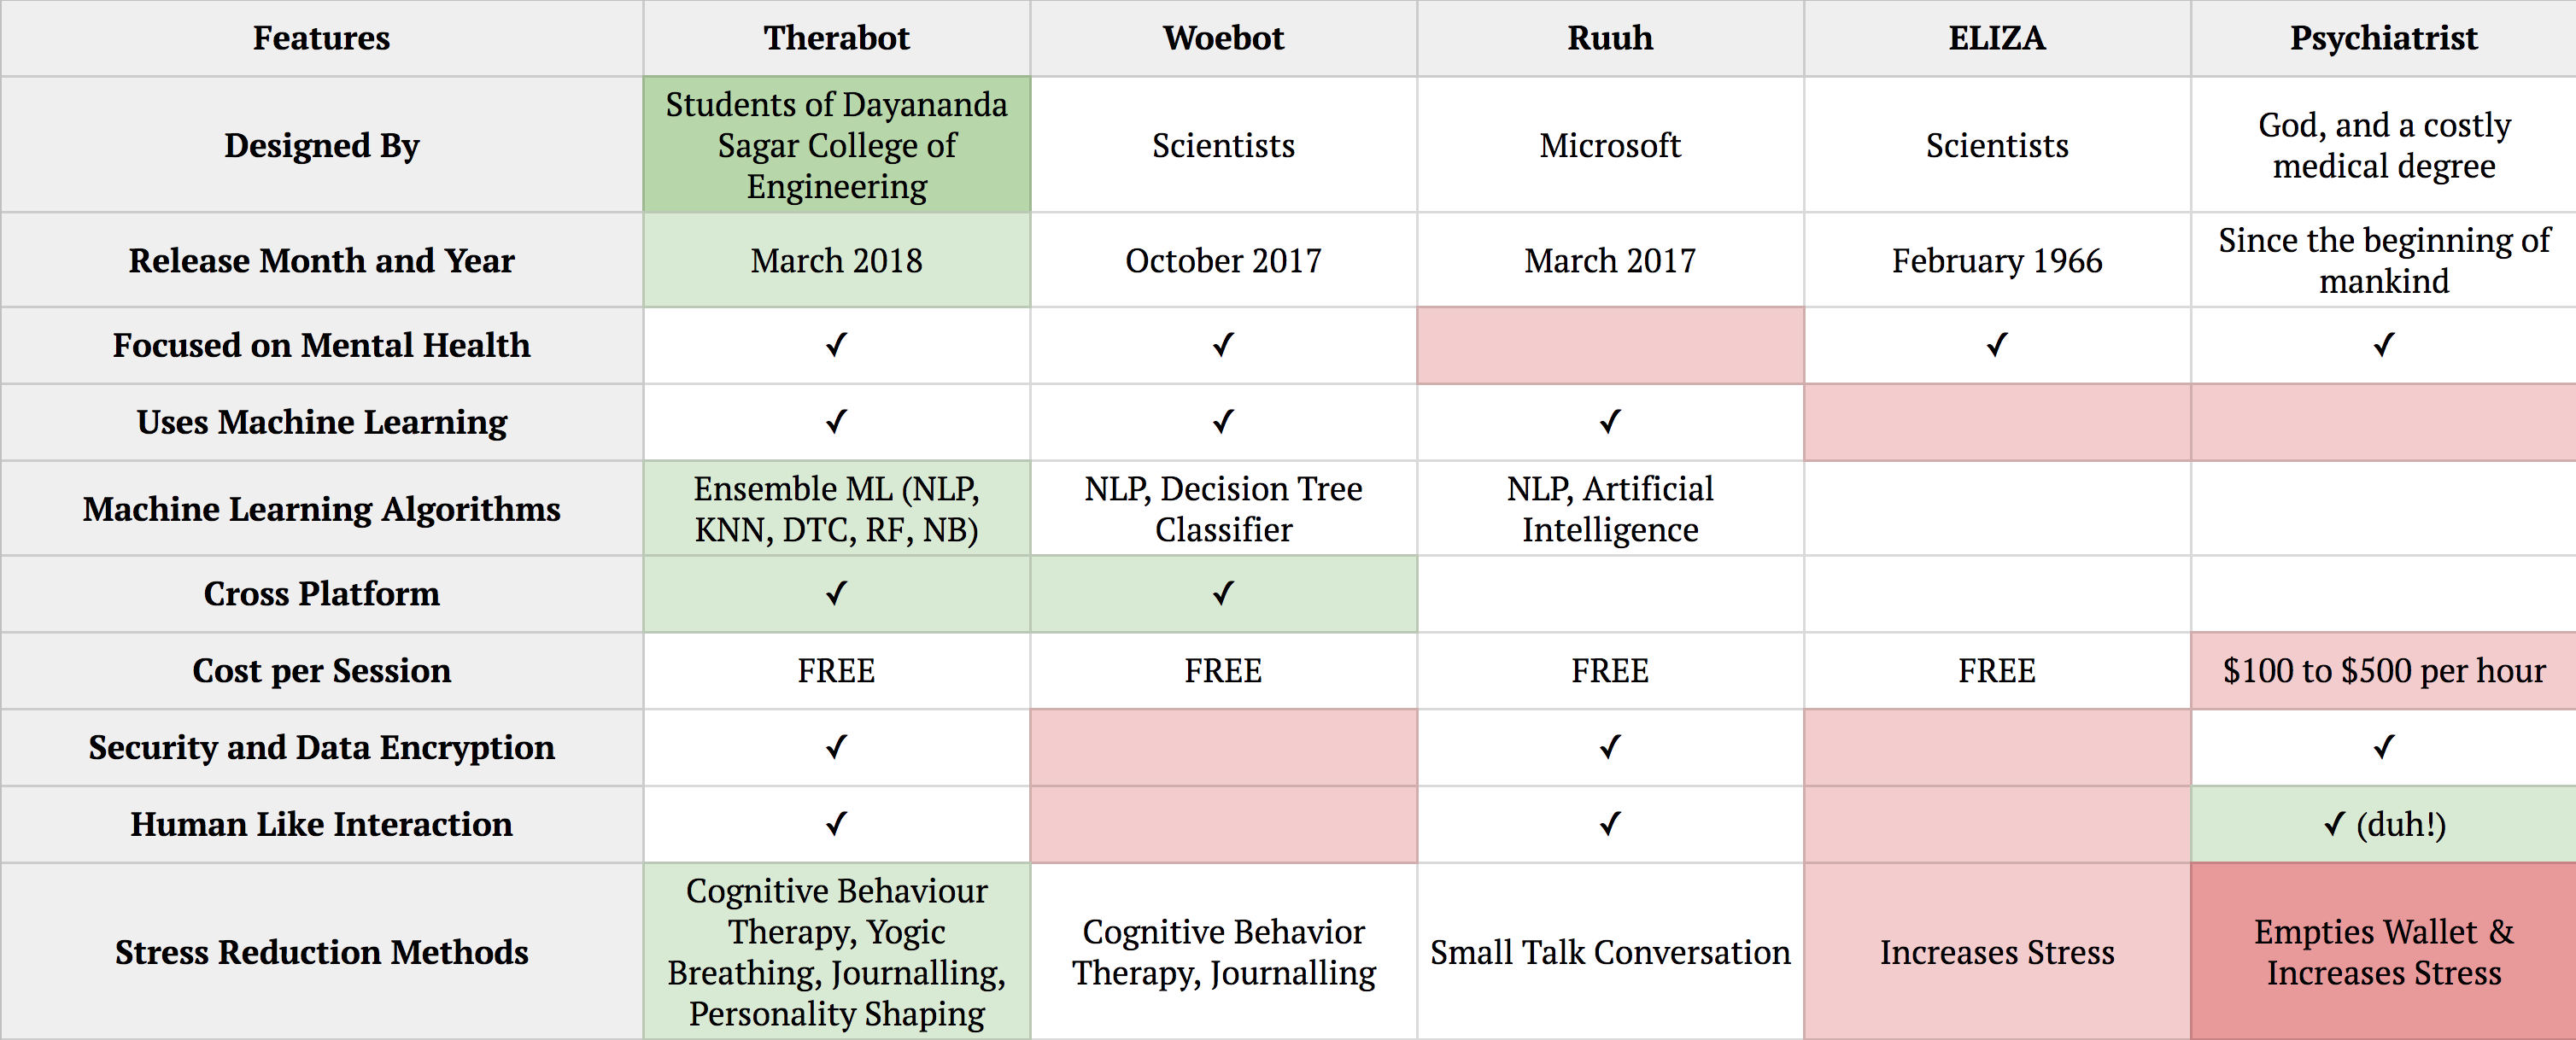
\includegraphics[width=\linewidth]{images/comparitive-study-of-competitors.png}
    \caption{Comparitive Study of Competitors}
    \label{fig:comparitive-study-of-competitors}
\end{figure}

Currently, people who do feel sad have only a handful of options available to them, including talking to friends, talking to family or seeing a therapist. The two are subjective, and doesn’t really apply when someone is clinically depressed and not willing to talk it out to his/her nearest and dearest.

Then, there are those who are hesitant to talk to strangers as well, considering they have the time and money to book an appointment with a therapist. Even if they do so, they have trouble opening up to someone who they have never met before.

When it comes to the existing Chatbot ecosystem, it has boomed in the market just a few days ago and has been dominant amongst companies to work as a front for their customer services portals, replacing everyday queries etc. We wanted to extend this functionality into something even more helpful and personal.

(why therapy, why chatbots) = (how good have they been : they trick the user into thinking that they are communicating with an actual person) chatbot which automatically gives immediate responses to the users based on the data set of Frequently Answered Questions (FAQs), using Artificial Intelligence Markup Language (AIML) and Latent Semantic Analysis (LSA). Template based questions like greetings and general questions will be answered using AIML and other service related questions use LSA to give responses.

\section{Proposed Solution}

The purpose of this study is to take an in-depth critical look into the narrative practice of externalizing; focusing intimately on its various uses and purported therapeutic qualities. The oneness of this deliberation is in the singular idiosyncrasy in which it locus on the various shot in which externalizing praxis are employed within narrative therapy and the leeway to which they are evaluated through research.

Narrative therapy proffer vast innovative essence and therapeutic practices. Key betwixt them is the praxis of engaging people in externalizing gab. Intermittently viewed as matter-of-factly a therapy technique, externalizing practices address wider inference about how clinicians view the world, understand clients quandary, and by association, how clients view their self and their potentiality to make turnover in their lives.

An evolving frame of narrative-inspired literature and research is being ordain that may assist in repose narrative therapy alongside other catalog and researched therapeutic entrance. An nonpartisan of this study is to further that literary process, concretely as it relates to the practice of externalizing. This study’s oneness lies in the comportment in which it targets solely on the issues and therapeutic entanglement surrounding externalizing practices. By doing this, it represents novel work in the field of narrative therapy literature, and will assist in explaining a pivotal narrative practice to the preponderant clinical psychology community.

The intent of this abstraction is to take an in-depth critical look into the narrative practice of externalizing; focusing intimately on its diversified uses and purported therapeutic qualities.

A considerable measure of literature abide on the multiple distinctive ways in which externalizing practices function. Much of the literature is sprinkled with various tantalizing therapeutic qualities ascribing to externalizing practices, often not beyond the context of how externalizing serves other narrative practices; such as deconstructive listening, reliant influence questions, discovering unique sequel, etc.

\pagebreak

Accordingly, the oneness of this study is in the singular manner in which it locus on the numerous ways in which externalizing practices are employed within narrative therapy and the leeway to which they are evaluated through research.

Narrative therapy affirms many innovative ideas and therapeutic convenance. Key among them is the process of engaging people in externalizing interactions. consistently it is viewed as simply, a therapy technique, externalizing practices address wider implications about how clinicians picture the world, understand clients’ problems, and by association, how clients view themselves and their ability to make a new revision to their lives.

While narrative-inspired texts discept externalizing practices to varying degrees, this study is distinguished by the manner in which it locus singularly on the use of and therapeutic value concord with externalizing practices. By doing so, this study provides a richer forbearing of the theory and convention of externalizing approaches to clinicians versed in narrative work, as well as to those new to the narrative advent. It also intends an opportunity to explore in-depth the sequence of research behind narrative therapy and externalizing practices.

\subsection{Unique Features}

\begin{itemize}
    \item Build a simple and interactive real time chat system.
    \item Extraction of preferences and interests of the user.
    \item Dedicated system which is able be a bolster of support and understanding.
    \item Designed in such a way that it should work in cross platform devices.
    \item Effective hybrid models built on ensemble methods for reedy prediction.
    \item Can be easily integrated and upgradable.
\end{itemize}

\pagebreak

\section{System Requirements}

\begin{itemize}
    \item Android/iOS Mobile Device to test/run the chatbot
    \item Facebook Messenger or Google Assistant
    \item Adequately fast Internet connection to access
    \begin{itemize}    
        \item Dialogflow
        \item Actions on Google Dashboard
        \item Firebase Firestore Database
        \item Google Cloud Platform Dashbaord
    \end{itemize}
    \item Node and NPM to run the webhook server
    \item Python 3.6+ to run the NLP and Analytics module
    \item iPython Notebook to test/run the scripts
    \item Flask to run the API server to access Python scripts
\end{itemize}